\documentclass{beamer} 
\usetheme{default} 
\usecolortheme{albatross}
\setbeamercovered{transparent}
%\useoutertheme{umbcfootline} 
%\setbeamertemplate{background canvas}[vertical shading][bottom=red!20,top=yellow!30] 


\usepackage[spanish]{babel}
%\usepackage[latin1]{inputenc}
\usepackage[utf8x]{inputenc}
\usepackage{multicol}


\title{Tipos de datos en Java}

\author{Manuel J. Molino Milla \and Luis Molina Garzón}

\date{\today} %

\institute{IES Virgen del Carmen \and Departamento de Informática}




%\beamerdefaultoverlayspecification{<+->}

\begin{document}


\begin{frame}
  \titlepage
\end{frame}

\begin{frame}
    \frametitle{Logo}
\begin{figure}

\includegraphics[scale=1]{imagenes/logo.jpeg} 
\caption{Logo Java}
\end{figure}
\end{frame}

\begin{frame}
  \frametitle{Contenido}
\begin{footnotesize}
  \tableofcontents[pausesections]
\end{footnotesize}\end{frame}


\section{Variables}

\begin{frame}[fragile]
    \frametitle{Variables}
    \framesubtitle{Programa que calcula el area de un círculo:}
    \begin{verbatim}
public class ComputaArea {
  public static void main(String[] args) {
    // Paso 1: Lee el radio
    // Paso 2: Computa area 
    // Paso 3: Muestra el area
  }
}
\end{verbatim}
\pause
\begin{itemize}[<+-| alert@+>]
      \item El programa necesita leer el radio que introduce el usuario por teclado.
      \item Luego hay que almacenar ese valor en algún lado.
	\item ¿Dónde se almacenará dicho valor?
\end{itemize}
\pause
\end{frame}
%hay que cambiar esto
\begin{frame}
    \frametitle{Variables}

\begin{itemize}[<+-| alert@+>]
      \item Es un lugar de memoria donde se almacena:
      \item Datos.
      \item Resultados de computar datos.
      \item Se identifican por un nombre, para acceder a esa posición de memoria.
      \item Se puede usar distintos nombres, en el caso anterior puede ser \emph{x} e \emph{y} para el radio y el area.
      \item Pero mejor usar palabras como \emph{radio} y \emph{area}
      \item Veremos variables de varios tipos:
      \item \emph{Tipos primitivos} como enteros, números decimales, caractéres o booleanos.
      \item O clases que van a definir nuevos tipos de datos.    
      \item Se llaman variables porque su valor puede \emph{variar} a lo largo del programa.
    \end{itemize}
    \pause

\end{frame}
%finish

\begin{frame}[fragile]
    \frametitle{Variables}
    \framesubtitle{Programa que calculo el area de un círculo:}
    \begin{verbatim}
public class ComputeArea {
   public static void main(String[] args) {
   double radio; // Declaramos el radio
   double area; // Declaramos el  area
   //Asignamos el radio
   radio = 20; // nuevo valor para el radio
   // Computamos el  area
   area = radio * radio * 3.14159;
   // Mostramos los resultados
   System.out.println("El area del círculo de radio " +
   radio + " es " + area);
   }
}
\end{verbatim}
\pause
\begin{itemize}[<+-| alert@+>]
      \item Usamos palabras reservadas para indicar el tipo de variable.
      \item En este caso usamos la variable de tipo \emph{double} para declarar el radio y el area.
\end{itemize}
\pause

\end{frame}

\begin{frame}
    \frametitle{Variables}

\begin{itemize}[<+-| alert@+>]
      \item En la declaración de variables decimos al compilador tanto el nombre como el tipo de dato.
      \item De esta manera el compilador reservara espacio suficiente en memoria para almacenar dicha variable.
      \item La sintaxis es: \emph{tipo\_dato variable}.
      \item Ejemplo:
      \item \emph{int contador; //declaramos un contador como entero}.
      \item \emph{double area; //declaramos como decimal a area}
      \item \emph{double tipoInteres; //declaramos como decimal el tipo de interes} 
      \item Por convención el nombre de variable va en minúscula (contador, area, tipoInteres, \dots).    
      \item En el caso de una palabra compuesta, se concatenan capitalizando la primera letra del resto de palabras (tipoInteres, areaCirculo, consumoGasSemanal, \dots)
      \end{itemize}
      \pause

\end{frame}

\begin{frame}
    \frametitle{Variables}

\begin{itemize}[<+-| alert@+>]
	\item Se pueden declarar varia a la vez:
	\item \emph{int i, j, k;}
      \item Existe la notación húngara donde la primera letra hace referencia al tipo de dato:
      \item Ejemplo:
      \item \emph{int iContador; //declaramos un contador como entero}.
      \item \emph{double dArea; //declaramos como decimal a area}
      \item \emph{double dTipoInteres; //declaramos como decimal el tipo de interes} 
      \item Es muy conveniente su incialización en el momento de su declaración:
      \item \emph{int contador=0; //declaramos un contador como entero}.
      \item \emph{double area=0; //declaramos como decimal a area}
      \item \emph{double tipoInteres=2.2; //declaramos como decimal el tipo de interes} 
      \end{itemize}
      \pause

\end{frame}

\begin{frame}
\frametitle{Tabla de símbolos}
\begin{itemize}[<+-| alert@+>]
\item Es una estructura de datos usada por el compilador para asociar a cada símbolo del programa fuente (variables, constantes, \dots)
\item Está formado por registros que contiene información tal y como:
\begin{enumerate}
\item Nombre del símbolo.
\item Dirección de memoria.
\item Tipo de dato.
\item Número de linea de la declaracíon o números de linea en los que se usa el símbolo. 
\end{enumerate}
\end{itemize}
\pause
\end{frame}


%\section{Todo es un objeto}

%\%subsection{Introducción}

%\begin{frame}
%    \frametitle{Introducción}

%\begin{itemize}[<+-| alert@+>]
%      \item Java es un lenguaje orientado a objetos \alert{puros}
%      \item C++ y Java es un lenguaje hibrido.
%      \item Permite varios estilos de programacion.
%      \item C++ permite la compatibilidad hacia atras con el lenguaje C.
%      \item En Java se asume que se desea realizar \emph{POO}      
%    \end{itemize}
%    \pause

%\end{frame}

%\begin{frame}eferencia).
%      \item Ademas la referencia (mando a distancia) puede existir por si solo.
%      \item Ejemplos:
%      \begin{enumerate}[<+-| alert@+>]
%		\item String s; //crea solo la referencia
%		\item String s= ``asdf''; //Creacion de referencia y objeto (buena praxis)
%		\item String s= new String (``asdf''); //Creacion de referencia y objeto 
%    \frametitle{Referencias}
%\begin{itemize}[<+-| alert@+>]
%      \item Todo \emph{objeto} se manipula mediante \emph{referencias}.
%      \item Simil: una television (objeto) se manipula con un mando a distancia (la r

%	\end{enumerate}
%    \end{itemize}
%    \pause

%\end{frame}

\begin{frame}
    \frametitle{Almacenamiento}

\begin{footnotesize}
\begin{description}[<+->]
      \item[Registros] Dentro del procesador, son rápidos y son escasos. No se tienen el control sobre ellos.
      \item[Pila] Reside en memoria RAM. Se mueve hacia abajo para crear memoria y de nuevo hacia arriba para liberarla. Cuando se compila se sabe el tamaño exacto y la vida de los datos almacenados en la pila. Aquí se crean las \emph{referencias} y \emph{NUNCA} los objetos.
      \item[Montículo] Reside en memoria RAM, el compilador \emph{NO} sabe cuanta memoria necesita o cuanto tiempo reside en memoria. Cada vez que se crea un objeto \emph{(new)} se asigna espacio. Lleva mas tiempo asignar espacio en el \emph{montículo que en la pila}
      \item[Almacenamiento estático] De ubicación o posición fija en RAM. Contiene datos que están disponibles durante todo el tiempo de ejecución. Se usa la palabra \emph{static} para asignar este espacio.
      \item[Almacenamiento no-RAM] Puede ser que los datos estén fuera del programa (incluso cuando no se ejecuta el programa) El truco consiste en convertir los objetos en algo que pueda existir en otro medio y que puedan recuperarse como objetos. \emph{stream y persistencia}
\end{description}
\end{footnotesize}

\end{frame}

\section{Tipos primitivos}

\subsection{Introduccion a tipos primitivos}

\begin{frame}
    \frametitle{Datos primitivos}

\begin{itemize}[<+-| alert@+>]
      \item Se usan con mucha frecuencia en un programa.
      \item No son objetos, no se crean con \emph{new}.
      \item Se suele usar el enfoque de C/C++.
      \item Se crean en una variable que no es una referencia.
      \item Dicha variable guarda el valor y lo coloca en la pila.
      \item Se consigue mas eficiencia.
      \item Java determina el tamaño de cada tipo primitivo, no variando de una plataforma a otra.      
    \end{itemize}
    \pause

\end{frame}

\subsection{Datos primitivos}

\begin{frame}
    \frametitle{Datos primitivos}
\begin{figure}
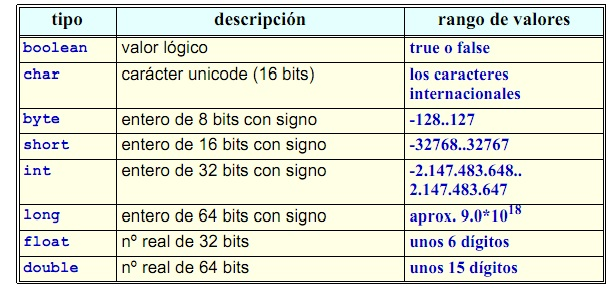
\includegraphics[scale=0.7]{imagenes/tipos_datos.jpg} 
\caption{Tipos de datos primitivos en Java}
\end{figure}

\end{frame}

\begin{frame}
    \frametitle{Enteros y reales}
\begin{block}{Numeros enteros y reales}
¿Cual es la diferencia entre numeros reales y enteros? Ejemplos.
\end{block}
\pause
\begin{block}{Ejemplos}
\begin{itemize}[<+-| alert@+>]
\item int interesBancario = 3; //interes aplicado
\item double interesBancario = 3.5; //interes aplicado
\item char letraDNI ='o'; //letra que acompaña al DNI
\item int velocidadLuz = 300000; //velocidad de la luz
\end{itemize}
\end{block}
\pause

\end{frame}

\begin{frame}
\frametitle{¿Como definimos los siguientes datos?}
\begin{itemize}[<+->]
\item Euribor 2.29\%
\item \emph{double euribor = 2.29;} 
\item Día de nacimiento
\item \emph{int diaNacimiento = 23;}
\item IVA 19\%
\item \emph{int iva= 19;}
\item Temperatura corporal 36 grados medidas en un termómetro clínico
\item \emph{double temperaturaCorporal = 36.0;}
\end{itemize}
\pause

\end{frame}

\subsection{Precisión}
\begin{frame}
\frametitle{Precisión}
\begin{block}{Mas de números}
\begin{itemize}[<+-| alert@+>]
\item¿Qué ocurre en el siguiente código? 
\item double precioUnitario=4.35;
\item double cantidad=100;
\item ¿Que produce la siguiente sentencia?
\item System.out.println(''Precio total: ''+precioUnitario*cantidad);
\end{itemize}
\end{block}
\pause
\begin{block}{Representacion digitos}
Los ordenadores trabajan en binario y a la hora de trabajar con variables de tipo float o double cometen errores de precisión al trabajar con valores que no pueden representar.
\end{block}
\pause

\end{frame}

\subsection{Tipo byte}
\begin{frame}
\frametitle{Tipo byte}
\begin{itemize}[<+-| alert@+>]
\item Es el tipo entero mas pequeño.
\item El rango va desde \emph{-128 a 127}
\item Son muy útiles cuando estamos trabajando con flujo de datos, por ejemplo con un fichero.
\item No se usan para realizar cálculos aritméticos.
\end{itemize}
\pause
\end{frame}

\subsection{Literales}
\begin{frame}
\frametitle{Literales}
\begin{itemize}[<+-| alert@+>]
\item Una literal es un valor constante formado por una secuencia de caracteres.
\item Son ejemplos de literales los números, los caracteres y las cadenas de caracteres. 
\item Números:
\begin{enumerate}
\item 123 //literal int
\item 123.456 //literal double
\item 123L //literal long
\item 123.456F //literal float
\end{enumerate}
\item Las literales boolenas consisten de las palabras reservadas \emph{true} y \emph{false}. 
\item Las literales de caracteres se expresan por un solo caracter entre comillas sencillas 'a', '\%', '5'
\item Literales de cadena que es una combinación de caracteres: ''hola'', ''1223'', ''cadena123''
\end{itemize}
\pause
\end{frame}

\begin{frame}
\frametitle{underscores}
\begin{itemize}[<+-| alert@+>]
\item Podemos usar el caracter \emph{\_} para declarar literales numéricos con mayor claridad.
\item Ejemplos:
\begin{enumerate}
\item long creditCardNumber = 1234\_5678\_9012\_3456L;
\item int millon = 1\_000\_000;
\item int billon = 1\_000\_000\_000\_000;
\end{enumerate}
\end{itemize}
\pause
\end{frame}

\begin{frame}
\frametitle{Ejemplo de literales}
\begin{figure}
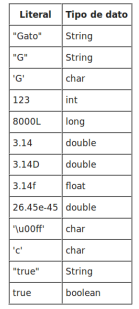
\includegraphics[scale=0.8]{imagenes/literales.png}
\end{figure}
\end{frame}

\begin{frame}

\frametitle{Ejercicio de literales}
\begin{verse}
Realiza un programa en el que definas distintos tipos de datos e inicializa dichos datos (dar un valor a la variable en el momento de la declaración). Utiliza en alguno de ellos underscore y finalmente muestra en pantalla su valor.
\end{verse}
\end{frame}

\subsection{Operadores}

\begin{frame}
    \frametitle{Operador asignación}
    Usamos \emph{=} Toma el valor de la parte derecha y lo copia en la parte izquierda. 	La asignacion de datos primitivos es sencilla.
    \pause
    \begin{footnotesize}
   
	\begin{block}{Los usamos en objetos}
	String referencia = new String(''Hola'');
	\end{block}
	\pause
	\begin{block}{Tipos primitivos}
	\begin{itemize}[<+-|alert@+>]
	\item int edad =25;
	\item double temperatura = 23.3;
	\item int cuadruple = numero*4;
\end{itemize}
	\end{block}
	\pause
	\begin{block}{¿Que resultado se obtiene?}
	\begin{itemize}[<+-|alert@+>]
		\item int A=5;
		\item int B=A;
		\item A=7;
		\item ¿Cual es el valor de A y B?
	\end{itemize}
	
	\end{block}
	 
    \end{footnotesize}
	\pause

\end{frame}

\begin{frame}
    \frametitle{Operadores}
\begin{figure}
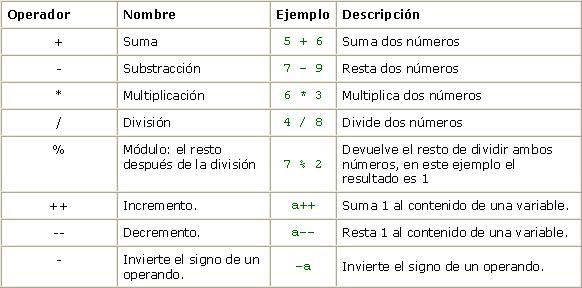
\includegraphics[scale=0.7]{imagenes/operadores.jpg} 
\caption{Operadores aritmeticos en Java}
\end{figure}
\end{frame}

\subsection{Precedencia o prioridad}
\begin{frame}
\frametitle{Precedencia o prioridad}
\framesubtitle{¿Que valores se obtienen en las siguientes expresiones aritmeticas?}
\begin{itemize}[<+->]
\item 5+3*2
\item \emph{11} 
\item 5*8+4/2*6-15+100/10
\item \emph{47}
\item -9*2+8*7-9-9/3
\item \emph{26}
\end{itemize}
\pause
\begin{itemize}[<+-|alert@+>]
\item Los operadores matemáticos tienen prioridades
\item El operador unario - tiene máxima prioridad -9*4
\item Le siguen * / \%
\item Posteriomente + y -
\item Para saltarnos las prioridades podemos usar paréntesis.
\end{itemize}
\pause

\end{frame}

\begin{frame}
\frametitle{Precedencia o prioridad}
\framesubtitle{¿Que valores se obtienen en las siguientes expresiones aritmeticas?}
\begin{itemize}[<+->]
\item 5+3*2
\item \emph{11} 
\item (5+3)*2
\item \emph{16}
\item -9*2+8*7-9-9/3
\item \emph{26}
\item -(9*2+8)*7-(9-9/3)
\item \emph{-188}
\item 6*4+(2-8*12)
\item \emph{-70}
\item 6*4+2-8*12
\item \emph{-70}
\end{itemize}
\pause
En caso de duda podemos usar los paréntesis, incluso puede ayudarnos a entender mejor la expresión matemática.
\end{frame}

\subsection{Autoincremento y autodecremento}
\begin{frame}
\frametitle{Operadores autoincremento y autodecremento}
\begin{itemize}[<+-|alert@+>]
\item El operador \emph{-}\emph{-} significa disminuir una unidad.
\item El operador \emph{++} significa aumentar una unidad.
\item \emph{++a} tiene igual sinificado que \emph{a=a+1}
\item \emph{-}\emph{-a} tiene igual sinificado que \emph{a=a-1}
\item Existe en version prefija \emph{-}\emph{-a} y \emph{++a}
\item Y en version postfija \emph{a-}\emph{-} y \emph{a++}
\end{itemize}
\pause

\end{frame}

\begin{frame}[fragile]
\frametitle{¿Qué salidas produce este programa?}
\begin{small}
\begin{verbatim}
public class Auto{
  public static void main(String[] args){
    int valorInicial1= 5;
    System.out.println(" valorInicial1++: "+ valorInicial1++);
    int valorInicial2=5;
    System.out.println(" ++valorInicial2: "+ ++valorInicial2);
    int valorInicial3=5;
    System.out.println(" valorInicial3--: "+ valorInicial3--);
    int valorInicial4=5;
    System.out.println(" --valorInicial4: "+ --valorInicial4);
    System.out.println("====================");
    System.out.println(" valorInicial1: "+ valorInicial1);
    System.out.println(" valorInicial2: "+ valorInicial2);
    System.out.println(" valorInicial3: "+ valorInicial3);
    System.out.println(" valorInicial4: "+ valorInicial4);
  }
}
\end{verbatim}
\end{small}
\end{frame}

\subsection{Asignación compuesta}
\begin{frame}
\frametitle{Asignación compuesta}
\begin{center}
\begin{large}
\begin{tabular}{|c|c|}
\hline
Operador&Significado\\
\hline
x += y&x = x+y\\
\hline
x -= y&x= x-y\\
\hline
x *= y&x =x*y\\
\hline
x /= y&x= x/y\\
\hline
x \%= y&x= x\%y\\
\hline
\end{tabular}
\end{large}
\end{center}
\end{frame}


\begin{frame}
\frametitle{Asignación compuesta}
\framesubtitle{¿Que valores se obtienen en las siguientes expresiones aritmeticas?}
El valor de x es 10 y el valor de y 3. Son valores de tipo int
\begin{itemize}[<+->]
\item x+=y
\item \emph{13} 
\item x-=y
\item \emph{7}
\item x*=y
\item \emph{30}
\item x/=y
\item \emph{3}
\item x\%=y
\item \emph{1}
\item x+=y*y
\item \emph{19}
\item x/=y*y
\item \emph{1}
\end{itemize}
\end{frame}

\subsection{Tipo caracter}
\begin{frame}
\frametitle{Tipo caracter}
\begin{itemize}[<+-|alert@+>]
\item Es el tipo \emph{char} empleado para representar caracteres simples.
\item ¿Qué es un caracter simple?
\item Se definen usando la palabra clave \emph{char} y encerrándolo entre comillas simples.
\item Ejemplo \emph{char letra = 'A';}
\item En el caso que declaremos de la siguiente forma:
\item \emph{''A''} no definimos un tipo \emph{char} sino un tipo \emph{string}
\end{itemize}
\pause

\end{frame}

\begin{frame}[fragile]
\frametitle{Unicode}
\begin{small}
\begin{itemize}[<+-|alert@+>]
\item Los computadores usan números binarios \emph{(0,1)} internamente.
\item Un caracter es almacenado como una secuencia de 0s y 1s
\item Llamamos codificar a mapear un caracter a su representación en binario.
\item Existen muchas formas de codificar un caracter según \emph{el esquema de codificación}, ejemplo \emph{ASCII} o \emph{Unicode}
\item Se usan 2 bytes para codificar \emph{(8 bits)}
\item Nos da la posibilidad de $2^{16}$ caracteres \emph{(65536)} 
\item Hoy en día se usan 1,112,064 caracteres usando \emph{caracteres suplementarios}
\item Usando el prefijo $\backslash u$ podemos usar notación hexadecimal y los valores van desde $\backslash u0000$ a $\backslash uFFFF$ 
\item Podemos asignar a la variable letra de tipo char el valor A de dos formas:
\item char letter = 'A';
\item char letter = $'\backslash u0041'$; 
\end{itemize}
\end{small}
\pause

\end{frame}

\begin{frame}
\frametitle{Caracteres especiales}
\begin{itemize}[<+-|alert@+>]
\item ¿Qué ocurre con la siguiente sentencia?
\item System.out.println(''He said ''Java is fun'''');
\item El compilador se queja. 
\item Java usa la secuencia de escape para usar caracteres especiales.
\item Se usa como secuencia de escape $\backslash$
\item System.out.println(''He said $\backslash$''Java is fun$\backslash$'''');
\end{itemize}
\pause

\end{frame}

\begin{frame}
\frametitle{Caracteres especiales} 
\begin{figure}
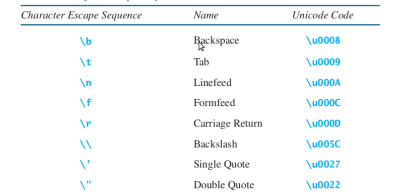
\includegraphics[scale=0.9]{imagenes/escape.png} 
\caption{Secuencias de escape en Java}
\end{figure}
\pause
 
\end{frame}


\begin{frame}
\frametitle{Tipo String}
\begin{itemize}[<+-|alert@+>]
\item El tipo \emph{char} representa un solo caracter.
\item Para representar una cadena de caracteres se usa el tipo \emph{String}
\item El tipo \emph{string} no es un tipo primitivo.
\item Representa objetos.
\item Usamos una referencia \emph{String nombre;} que se almacena la pila de memoria.
\item Posteriormente creamos un objeto: \emph{nombre=''Federico''}
\item O bien \emph{nombre = new String(''Federicio'')}
\item O también \emph{String nombre= new String(''Federico'');}
\item Dicho objeto se almacena en el montículo de la memoria.
\end{itemize}
\pause

\end{frame}

\subsection{Convesión de tipos}
\begin{frame}
    \frametitle{Convesión de tipos}
Podemos convertir los tipos entres si, de entero a doble, de doble a entero, \dots

        \pause
	\begin{block}{Conversiones implícitas}
	\begin{itemize}[<+-|alert@+>]
		\item Se realizan de forma automática.
		\item Requiere que la variable destino (izquierda) tenga mayor precisión que la de la derecha.
		\item int x=12; double y = x; y vale 12.0
	\end{itemize}
	\end{block}
	\pause
	\begin{block}{Conversiones explícitas}
	\begin{itemize}[<+-|alert@+>]
	\item Hay que forzar dicha conversion.
	\item Se da en el caso que la variable de la derecha tenga menos precision que la de la izquierad.
	\item double x= 19.4;
	\item int y = (int) x; ahora y vale 19
\end{itemize}
	\end{block}
\end{frame}

\begin{frame}
\frametitle{Conversión de tipos}
\framesubtitle{¿Que valores se obtienen en las siguientes expresiones aritmeticas?}
\begin{footnotesize}
\begin{itemize}[<+->]
\item int x=7; double y=13.4; x+=(int)y;
\item \emph{20} 
\item double x=7.5; int y=13; x-=y;
\item \emph{-5.5}
\item int x=2; double y=2E1; x*=(int)y;
\item \emph{40}
\item double x=5.5; int y=2; x/=y;
\item \emph{2.75}
\item int x=56; double y=10.2; x\%=(int)y;
\item \emph{6}
\item float x=1.1F; double y=3.0; x+=y*y; ¿correcto?
\item \emph{10.1 de tipo float}
\item double x=1.1; float y=3.0F; x+=y*y; ¿correcto?
\item \emph{10.1 de tipo double}
\item int x=1; long y=3; x+=y*y; ¿correcto?
\item \emph{10 de tipo int}
\item long x=1; int y=3; x+=y*y; ¿correcto?
\item \emph{10 de tipo long}
\end{itemize}
\end{footnotesize}
\end{frame}


\subsection{Operadores de bits}
\begin{frame}
\frametitle{Operadores de bits}
\begin{itemize}[<+-| alert@+>]
\item Los datos en una computadora internamente se representan en código binario.
\item El microprocesador solo entiende de ceros y unos.
\end{itemize}
\begin{figure}
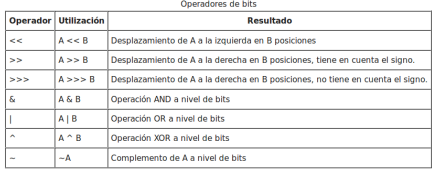
\includegraphics[scale=0.8]{imagenes/operadorbit.png}
\end{figure}
\end{frame}


\begin{frame}[fragile]
\frametitle{Ejemplo de operadores de bits}
Desplazamiento hacia la izquierda
\begin{verbatim}
int j = 33;
int k = j << 2;
...........................
00000000000000000000000000100001 : j = 33
00000000000000000000000010000100 : k = 33 << 2 ; k = 132   
\end{verbatim}
\pause
Desplazamiento hacia la derecha
\begin{verbatim}
int k = 132;
int m = k >> 2;
...........................
00000000000000000000000010000100 : k = 132    
00000000000000000000000000100001 : m = 132 >> 2 ; m = 33
\end{verbatim}
\end{frame}


\subsection{Constantes}
\begin{frame}
\frametitle{Constantes}
\begin{block}{Ejemplos}
\begin{itemize}[<+-| alert@+>]
\item public final static double PI =3.1416;
\item public final static int IVA =16;
\end{itemize}
\end{block}
\pause
\begin{block}{Explicación}
\begin{itemize}[<+-| alert@+>]
\item Se definen \emph{public} para que se pueda acceder desde cualquier sitio.
\item \emph{final} la identifica como una constante. Al ser constantes y no variables nos aseguramos que su valor no se va modificar.
\item \emph{static} indica que solo existe una copia en el programa. 
\item Finalmente se indica el tipo de dato, el nombre \emph{EN MAYUSCULA} y se le asigna su valor.
\end{itemize}
\end{block}
\pause

\end{frame}

\subsection{Tipo enum}
\begin{frame}[fragile]
\frametitle{enum en Java}
\begin{itemize}[<+-| alert@+>]
\item A partir de la versión 5 de Java se incorporarón al lenguaje los tipos de datos enumerados.
\item Un enum en Java es un conjunto fijo y relacionado de constantes.
\item Los enums se definen de la siguiente forma:
\end{itemize}
\pause
\begin{small}

\begin{verbatim}
// Guardamo en un archivo llamado Dia.java
public enum Dia {
 LUNES, MARTES, MIERCOLES, JUEVES, VIERNES, SABADO, DOMINGO
}
\end{verbatim}
\end{small}
\pause
\begin{verbatim}
// Ejemplo de uso:
Dia dia = null;
if (dia == Dia.DOMINGO)
  System.out.println("Día festivo");
\end{verbatim}
\pause
\end{frame}

\section{Generalidades }
\subsection{Sentencias} 

\begin{frame}
    \frametitle{Sentencias}
\begin{block}{Definicion de sentencias}
\begin{itemize}[<+-| alert@+>]
\item Cada una de las lineas que definimos en un programa se llaman \emph{sentencias}
\item Generalmente las sentencias se acaban en punto y coma:
\begin{enumerate}
\item char letraDNI ='o'; 
\item String palabra = new String(''palabra'');
\item System.out.println(palabra);
\item final static double PI = 3.1416;
\item import java.util.Scanner;
\item return valor;
\item valor++;
\item this.nombre=nombre;
\item System.out.printf(''\%+d \%n'', x);
\end{enumerate} 
\end{itemize}
\end{block}
\pause

\end{frame}

\subsection{Comentarios} 

\begin{frame}
    \frametitle{Comentarios}
    \begin{block}{Comentarios de una linea}
	System.out.println ("Hola mundo"); //esto es un comentario
    \end{block}
    \pause
\begin{block}{Comentarios de varias lineas}
/* Todo esto \\
   también es un\\
   comentario */\\
public void unMedodo (int unParametro)
    \end{block}
    \pause
    \begin{block}{Comentarios que genera documentacion}
/** Todo esto\\
   también es otro\\
   comentario */\\
public void unMedodo (int unParametro) \dots
    \end{block}
    
\end{frame}

\subsection{Ámbito de variables}
\begin{frame}
\frametitle{Ambito de variables}
El ámbito o alcance de una variable es la zona del programa donde la variable es accesible.
\begin{description}[<+-| alert@+>]
\item[Variables miembro o atributos de una clase] Son las declaradas dentro de una clase. Son accesibles en cualquier método de la clase
\item[Variables locales] Son las declaradas dentro de un método. Están disponibles desde su declaración hasta el final del método donde se declaran.
No son visibles desde otros métodos. Se crean en memoria cuando se declaran y se destruyen cuando acaba la ejecución del método.
\item[Variables de bloque]  Son las declaradas dentro de un bloque de instrucciones delimitado por llaves \{ \}. Su ámbito comienza en el punto donde se declara la variable. Están disponibles desde su declaración hasta el final del bloque donde se declaran. No son visibles desde otros bloques.
\end{description}
\pause

\end{frame}

\begin{frame}
\frametitle{Ámbito variables} 
\begin{figure}
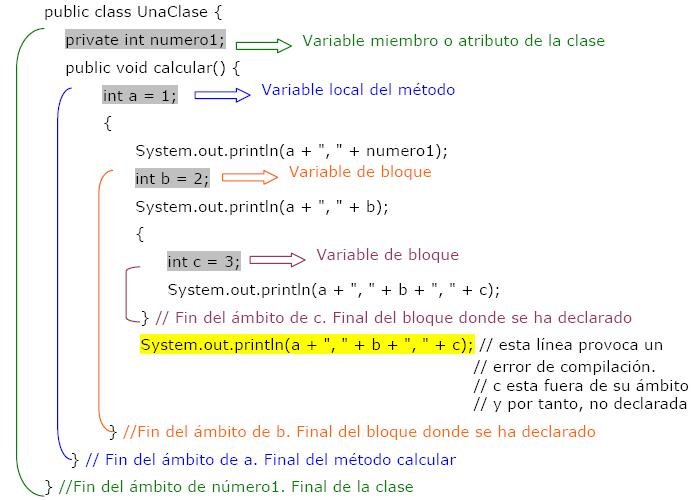
\includegraphics[scale=0.55]{imagenes/ambito.jpg} 
\caption{Ejemplo ambito variables Java}
\end{figure} 
\end{frame}

\subsection{Estilos de programación}
\begin{frame}[fragile]
\frametitle{Indentación} 
\begin{small}
\begin{multicols}{2}
\begin{block}{Sin indentacion}
\begin{verbatim}
public class Alumno{
private String nombre;
Alumno(String nombre){
this.nombre=nombre;
}
public String getNombre(){
return nombre;
}     
}
\end{verbatim}
\end{block}
\pause
\begin{block}{Con indentación}
\begin{verbatim}
public class Alumno{
   private String nombre;
   Alumno(String nombre){
      this.nombre=nombre;
   }
   public String getNombre(){
      return nombre;
   }     
}
\end{verbatim}
\end{block}
\end{multicols}
\end{small}

\end{frame}

\begin{frame}[fragile]
\frametitle{Estilos de bloque} 
\begin{small}
\begin{multicols}{2}
\begin{block}{Siguiente linea}
\begin{verbatim}
public class Alumno
{
   private String nombre;
   Alumno(String nombre)
   {
      this.nombre=nombre;
   }
   public String getNombre()
   {
      return nombre;
   }     
}
\end{verbatim}
\end{block}
\pause
\begin{block}{Final de linea}
\begin{verbatim}
public class Alumno{
   private String nombre;
   Alumno(String nombre){
      this.nombre=nombre;
   }
   public String getNombre(){
      return nombre;
   }     
}
\end{verbatim}
\end{block}
\end{multicols}
\end{small}

\end{frame}

\begin{frame}
\frametitle{Preguntas} 
\begin{figure}

\includegraphics[scale=0.9]{imagenes/dudas.png} 
\caption{Lenguaje máquina}
\end{figure} 
\end{frame}



\end{document}

